\documentclass[../stats.tex]{subfiles}
\graphicspath{{\subfix{../figures/}}}
\begin{document}
\chapter{Sampling Distributions}
\section{Sampling Distributions of Sample Proportions}
I have a bag of beads - we are interested in the true proportion of purple beads in your population (bag).
\begin{itemize}
    \item $n$ = population size = 50
    \item $p$ = population proportion = true prop. of purple beads = ?
\end{itemize}

You received a bag of 50 beads. You will perform 20 trials of this experiment.
\begin{enumerate}
    \item Mix the bag well before collecting each sample.
    \item Without looking, randomly select 5 beads from your bag (without replacement).
    \item Count the number of purple beads in your sample and record a tally in the appropriate column below.
\end{enumerate}

Here is the data 
\begin{center}
    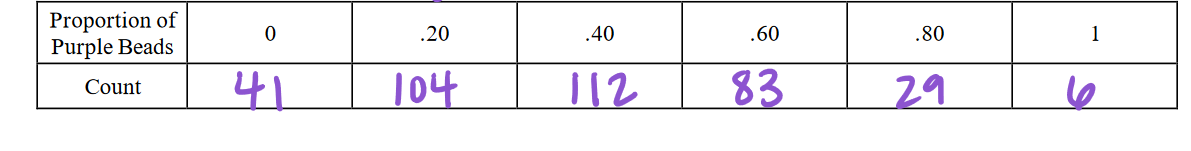
\includegraphics[width=0.8\textwidth]{5.1.1.PNG}
\end{center}

Sampling Distribution of the data 
\begin{center}
    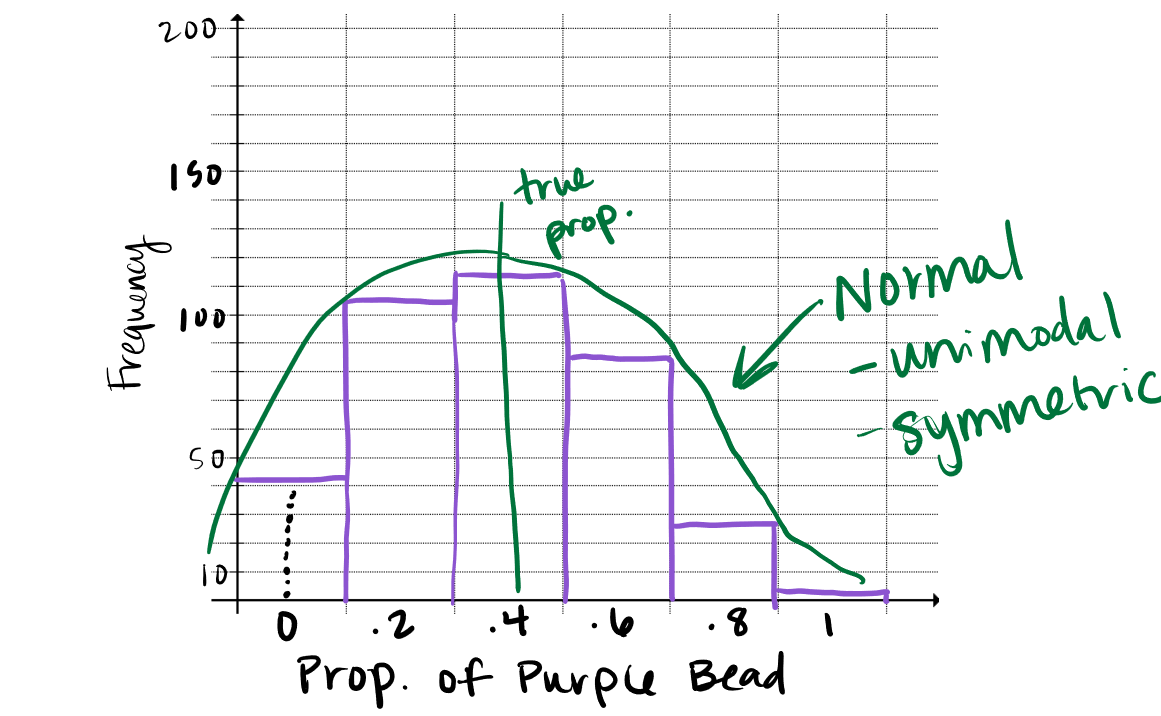
\includegraphics[width=0.8\textwidth]{5.1.2.PNG}
\end{center}

As we begin to use sample data to draw conclusions about a larger population, we must be clear about whether a number describes a sample or a popluation.
\begin{itemize}
    \item Parameter: is a number that describes some characteristic of a population 
    \item Statistics: is a number that describes some characteristic of a sample 
    \item Unbiased Estimator: a sample proportion or sample mean that is equal to the population proportion or population mean 
\end{itemize}
\begin{center}
    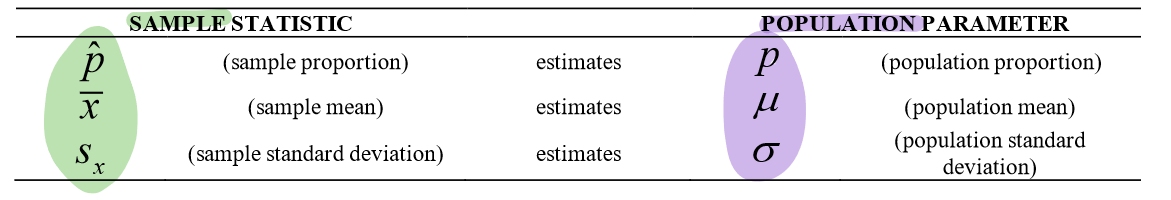
\includegraphics[width=0.8\textwidth]{5.1.3.PNG}
\end{center}

Rather than showing real repeated samples, imagine what would happen if we were to actually draw many samples. Now imagine what would happen if we looked at the sample proportions for these samples.
The histogram we'd get if we could see all the proportions from all possible samples is called the sampling distribution of the sample proportions.

What would the histogram of all the sample proportions look like?
\begin{itemize}
    \item We would expect the histogram of the sample population to center at the true population, $p$, in the population.
    \item The spread is calculated as standard deviation based on the true proportion, $p$, and teh sample size, $n$. As the sample size gets larger the standard deviation will get smaller.
    \item The shape of the histogram would be unimodal and symmetric.
    \item More specifically, a normal model is just the right one for the histogram of sample proportions.
\end{itemize}

Assumptions and Conditions 
\begin{itemize}
    \item Randomness: The sample should be a simple random sample of the population. This allows us to calculate mean.
    \item Independence (10\% Condition): The sample size, $n$, must be no larger than 10\% of the population. 
    
    Basically, population $\geq 10n$. This allows us to calculate standard deviation.

    \item Normality (Large Counts Condition): The sample size has to be big enough so that both number of successes and number of failures is at least 10. We also refer to this as the Success/Fail Condition.
    
    Success: $np\geq 10$, Fail: $n(1-p)\geq 10$. This allows us to call our sampling distribution approximately normal.
\end{itemize}

Provided that the sampled values are independent and the sample size is large enough, the sampling distribution of $p$ is modeled by a normal model with:

Sample Proportions: $\hat{p}=\frac{\#{\text{successes}}}{\text{sample size}}$

Mean of Sample Proportions: $\mu_{\hat{p}}=p$

Standard Deviation of Sample Proportions: $\sigma_{\hat{p}}=\sqrt{\frac{p(1-p)}{n}}$

Where $p$ is population proportion, and $n$ is sample size.

\pagebreak
\begin{example}
    A recent study looked at the percentage of young adult women who get less than 7 hours of sleep a night. In this study, they say that 45\% of women get less than 7 hours of sleep a night.
    What is the probability that a random sample of 50 women will result in a sample proportion of 50\% or higher?

    (a) Communicate the parameter in the context of the problem.

    $p$ = true proportion of women who get less than 7 hours of sleep per night.

    (b) Create the sampling distribution by finding the center, spread, and shape. Make sure to check each condition first.

    Random: Random sample of 50 women, $\mu_{\hat{p}}=0.45$

    Independent: Assume $n=50\leq 0.10$(all young women), $\sigma_{\hat{p}}=\sqrt{\frac{9.45(1-0.45)}{50}}=0.0704$

    Normal: $50(0.45)=22.5\geq 10$, $50(0.55)=27.5\geq 10$, sampling distribution is approximately normal.

    (c) Calculate the probability by converting your data to a z-score and using normalcdf to find the probability.

    $P(\hat{p}\geq 50)=P(z\geq 0.7102)$. normalcdf(lower: 0.7102, upper: $\infty$, $\mu: 0$, $\sigma:1$) = 0.2388.

    (d) Conclude the problem by answering the question in a complete sentence with the context of the problem.

    When the true proportion of young women who sleep less than 7 hours is 45\%, the probability a random sample of 50 women results in a sample proportion of 50\% or higher is approximately 23.89\%.
\end{example}

\begin{example}
    Percy fails to study for his chemistry final. The final has 100 multiple choice questions, each with five choices. Assume all questions are independent and that Percy has given himself over the gods of chance and randomly guesses on each of the 100 questions.

    (a) What is the parameter in the context of the problem.

    $p$ = true proportion of questions Percy gets correct 

    (b) Identify $n$ and $p$ for this problem.

    $n=100$, $p=0.20$

    (c) Is the sampling distribution approximately normal? Why or why not?

    $100(0.20)=20\geq 10$, $100(0.80)=80\geq 10$. Sampling distribution is approximately normal.

    (d) Is the sampling distribution unbiased? Why or why not?

    Because each question is randomly guesses, it is unbiased.

    (e) Do we have to check the 10\% condition here? Why or why not?

    It is stated that each guess is independent, so there is no need to check.

    (f) Calculate the mean and standard deviation for this problem.

    $\mu_{\hat{p}}=0.20$, $\sigma_{\hat{p}}=\sqrt{\frac{.20(1-.20)}{100}}=0.04$

    (g) What is the probability that Percy will get between a 25\% and a 50\% on the test? Show all work.

    $z$-score for $0.25$ = 1.25, $z$-score for 0.50 = 7.5. 

    $P(1.25\leq z\leq 7.5)$ = normalcdf(lower: 1.25, upper: 7.5, $\mu:0$, $\sigma_1$) = 0.1056.

    When the true proportion of correct questions is 0.20, the probability Percy will get between a 25\% and 50\% on the test is 0.1056.
\end{example}


\section{Sampling Distributions of Sample Means}
The notation for means is the following:
\begin{itemize}
    \item Parameters: $\mu$ and $\sigma$
    \item Statistics: $\overline{x}$ and $s$
    \item Sampling Distribution Mean: $\mu_{\overline{x}}$
    \item Sampling Distribution Standard Deviation: $\sigma_{\overline{x}}$
\end{itemize}

Conditions for Sample Means 
\begin{itemize}
    \item Random - As long as the sampling method is random, our mean is an unbiased estimator.
    \item Independent - When sampling, we have to make sure the 10\% condition is satisfied.
    \item Normal - No longer checking Large Counts (Success/Fail)
\end{itemize}
Central Limit Theorem:
\begin{itemize}
    \item The central limit theorem (CLT) states that when the sample size is sufficiently large, a sampling distribution of the mean of random variable will be approximately normally distributed.
    \item The central limit theorem requires that the sample values are independent of each other and that $n$ is sufficiently large.
\end{itemize}

Therefore:
\begin{itemize}
    \item If the population distribution is normal, then so is the sampling distribution of $\overline{x}$. This is true no matter what the sample size $n$ is.
    \item If the population distribution is not normal (or has an unknown shape), the central limit theorem tells us that the sampling distribution of $\overline{x}$ will be approximately normaly in most cases of $n\geq 30$.
\end{itemize}

Samping Distributions for Sample Means:

Shape: Approximately Normal, as long as 
\begin{itemize}
    \item If $n<30$, the population distribution is normal.
    \item If $n\geq 30$, the CLT tells us the sampling distribution will be approximately normal.
\end{itemize}

Center: $\mu_{\overline{x}}=\mu$, as long as 
\begin{itemize}
    \item You randomly selected from the population of interest (sampling) or randomly assigned treatments (experiments).
\end{itemize}

Spread: $\sigma_{\overline{x}}=\frac{\sigma}{\sqrt{n}}$, as along as 
\begin{itemize}
    \item Your sample size is less than 10\% of the population of interest.
    \item You only use 10\% condition when sampling otherwise we will have to assume independence.
\end{itemize}

\pagebreak
\begin{example}
    Suppose the heights of young women are normally distributed with $\mu=64.5$ inches and $\sigma=2.5$ inches. What is the probability that the mean height of an SRS of 10 young women is greater than 65 inches?

    (a) Communicate the parameter in the context of the problem.

    $\mu$ = true average height of a young woman 

    (b) Create a sampling distribution by finding the center, spread, and shape. Make sure to check conditions!

    Random: SRS of 10 young women, $\mu_{\overline{x}}=64.5$

    Independence: Assume $n=10\leq 0.10$(all young women). $\sigma_{\overline{x}}=\frac{2.5}{\sqrt{10}}=0.7906$

    Normal: Population is normally distributed therefore the sampling distribution is normal.

    (c) Calculate the probability by converting your data to a z-score and finding the probability.

    $P(z>\frac{65-64.5}{.7906})=P(z>0.6324)$. 

    normalcdf(lower: 0.6324, upper: $\infty$, $\mu:0$, $\sigma:1$) = 0.2636.

    (d) Conclude by answering the question in a complete sentence with the context of the problem.

    When the mean height of young women is 64.5 inches, the probability of selecting an SRS of 10 young women with a mean height greater than 65 inches is 26.36\%.
\end{example}

\begin{example}
    A restaurant is suspected of undercooking its burgers. The restaurant claims that its burgers are cooked to a medium doneness, with an average internal temperature of 160 degrees Fahrenheit and a standard deviation of 5 degrees Fahrenheit.
    For the questions that follow, assume that the restaurant's claim is accurate and that the distribution of internal temperatures follows a normal distribution.

    (a) What is the probability that a single randomly selected burger is cooked to an internal temperature of 158 degrees or less.

    $P(x\leq 158)=P(z\leq \frac{158-160}{5})=P(z\leq -0.4)$. 

    normalcdf(lower: $-\infty$, upper: $-0.4$, $\mu:0$, $\sigma:1$) = 0.3446.

    (b) A secret shopper comes in at random times throughout the data to test the internal temperature of the burgers. They select an SRS of 25 burgers and calculate the sample mean. What are the mean and standard deviation of the resulting sampling distribution?

    Random: SRS Of 25 burgers. $\mu_{\overline{x}}=160$

    Independence: Assume $n=25\leq 0.10$(all burgers). $\sigma_{\overline{x}}=\frac{5}{\sqrt{25}}=1$

    (c) The secret shopper in part (b) obtains a sample mean of $\overline{x}=158$ degrees Fahrenheit. What is the probability that a random sample of 25 burgers produces a sample mean amount of 158 degrees or less? Assume all conditions are met.

    $P(\overline{x}\leq 158)=P(z\leq -2)$ = normalcdf(lower: $-\infty$, upper: $-2$, $\mu:0$, $\sigma:1$) = 0.0228.

    (d) Why is there a difference between the results of (a) and (c)? Explain why one is more likely to happen than the other.

    In Part (a) we are looking at the probability a single burger is 158 degrees or less, and since the distribution has more variability in it, we have a higher probability of it happening randomly. In part (c) we are looking at the probability that 25 burgers have an average 
    temperature of 158 degrees or less, and since averages have less variability than individual values, we haev a lower probability of it happening randomly.
\end{example}

\section{Combining Sample Proportions and Sample Means}
Creating sampling distributions of a difference in sample proportions will set us up for success when we study inferences in Unit 6.

These sampling distributions can be used to answer the common question of ``which is better?'' For example:
\begin{itemize}
    \item Which of two popular drugs - Lipitor or Pravachol - helps lower ``bad cholesterol'' more?
    \item Researchers used 4000 people with heart disease as subjects in a completely randomized experiment. They were randomly assigned to one of two treatment groups: Lipitor or Pravachol.
    \item At the end of the study, researchers compared the proportion of subjects in each group who had died, had a heart attack, or suffered other serious consequences within two years.
    \item For the subjects assigned to Pravachol, 0.263 suffered a serious consequence.
    \item For the subjects assigned to Lipitor, 0.224 suffered a serious consequence.
\end{itemize}

Does this mean that Lipitor is better at lowering bad cholesterol? Is this difference a result of Lipitor being better or is it merely due to a chance involved in the random assignment of treatments? Answers to these questions require a sampling distribution of a difference in sample proportions.

$\hat{p}_1$ will denote the sample proportion from the first group.

Center: $\mu_{\hat{p}_1-\hat{p}_2}=p_1-p_2$, as long as:
\begin{itemize}
    \item Both samples must have been randomly selected from the population (or involve random assignment for an experiment).
\end{itemize}

Spread: $\sigma_{\hat{p}_1-\hat{p}_2}=\sqrt{\left(\frac{p_1(1-p_1)}{n_1}\right) + \left( \frac{p_2(1-p_2)}{n_2}\right)}$ as long as 
\begin{itemize}
    \item Both samples satisfy the 10\% condition: 
    \[ n_1<0.10N_1 \]
    \[ n_2 < 0.10 N_2 \]
    \item If this is an experiment, check if it is safe to assume independence.
\end{itemize}

Shape: Approximately normal, as long as 
\begin{itemize}
    \item Both samples must satisfy the success/fail condition.
    \begin{center}
        $n_1p_1\geq 10$ and $n_1(1-p_1)\geq 10$ \\
        $n_2p_2\geq 10$ and $n_2(1-p_2)\geq 10$
    \end{center}
\end{itemize}

\pagebreak
\begin{example}
    A recent study examined the percentage of young adult women and men who get less than 7 hours of sleep a night. In this study, it was found that 45\% of women and 38\% of men get less than 7 hours of sleep a night. What is the probability that a random sample of 50 women and 75 men will result in a difference of 15\% or more between the groups?

    (a) State the parameters in the context of the problem.

    $p_w$: proportion of women who get less than 7 hours of sleep

    $p_m$: proportion of men who get less than 7 hours of sleep.

    (b) Create the sampling distribution by finding the center, spread, and shape. Make sure to check each condition first.

    Random: Random sample of 50 women and 75 men. $\mu_{\hat{p}_w-\hat{p}_m}=0.45-0.38=0.07$

    Independent: Assume $n_w=50\leq 0.10$(all women) and $n_m=75\leq 0.10$(all men).

    $\sigma_{\hat{p}_w-\hat{p}_m}=\sqrt{\frac{.45(.55)}{50}+\frac{.38(.62)}{75}}=0.0900$

    Normal: $50(.45)=22.5\geq 10$, $75(.38)=28.5\geq 10$, $50(.55)=27.5\geq 10$, $75(.62)=46.5\geq 10$. Sampling distribution is approximately normal.

    (c) Calculate the probability by converting your data to a z-score and using normalcdf to find the probability.

    $P(p_w-p_m\geq 0.15) = P(z\geq 0.8889) = 0.1870$

    $P(p_w-p_m\leq -0.15)=P(z\leq -2.4444) = 0.0073$

    (d) Conclude the problem by answering the question in the context of the problem.

    The probability that a random sample of 50 women and 75 men will result in a difference of 15\% or more getting less than 7 hours of sleep between the two groups is approximately $19.43\%$.
\end{example}

Sampling Distribution of $\overline{x}_1-\overline{x}_2$:

Center: $\mu_{\overline{x}_1-\overline{x}_2}=\mu_1-\mu_2$ as long as 
\begin{itemize}
    \item Both samples must have been randomly selected from the population (or involve random assignment for an experiment)
\end{itemize}

Spread: $\sigma_{\overline{x}_1-\overline{x}_2}=\sqrt{\frac{\sigma_1^2}{n_1}+\frac{\sigma_2^2}{n_2}}$ as long as 
\begin{itemize}
    \item Both samples satisfy the 10\% condition: 
    \[ n_1<0.10N_1 \] 
    \[ n_2 <0.10 N_2 \]
    \item If this is an experiment, check if it is safe to assume independence.
\end{itemize}

Shape: Approximately normal, as long as 
\begin{itemize}
    \item $n_1\geq 30$ and $n_2\geq 30$ to use the Central Limit Theorem (CLT), and if one or both are less than 30, each population should be normal.
\end{itemize}

\pagebreak
\begin{example}
    A study is conducted to compare the effectiveness of two study techniques, A and B, in inproving test scores. For Technique A, a random sample of 80 students yields an average score of 85 with a standard deviation of 10.
    For Technique B, a random sample of 100 students yields an average score of 82 with a standard deviation of 8. Calculate the probability that the difference in the average scores between Technique A minus Technique B is greater than 4.

    (a) State the parameters in the context of the problem.

    $\mu_A$: mean score of students using Technique A 

    $\mu_B$: mean score of students using Technique B 

    (b) Create the sampling distribution by finding the center, spread, and shape. Make sure to check each condition first.

    Random: Random sample of 80 Technique A and 100 Technique B Students. $\mu_{\overline{x}_A-\overline{x}_B} = 85-82=3$

    Independent: Assume $n_A=80\leq 0.10$(all technique A students) and $n_B=100\leq 0.10$(all technique B students). $\sigma_{\overline{x}_A-\overline{x}_B}=\sqrt{\frac{10^2}{80}+\frac{8^2}{100}}=1.3748$.

    Normal: $n_A=80\geq 30$, $n_B=100\geq 30$. CLT says sampling distribution will be approximately normal.

    (c) Calculate the probability by converting your data to a z-score and using normalcdf to find the probability.

    $P(\mu_{\overline{x}_A}-\mu_{\overline{x}_B} > 4) = P(z>0.7274) = 0.2335$.

    (d) Conclude the problem by answering the question in context of the problem.

    The probability that the difference in the average scores between Technique A and B is greater than 4 is approximately 23.35\$.
\end{example}

\end{document}